\documentclass[a4paper,10pt,smallheadings,twocolumn]{scrartcl}

\usepackage{times}
\usepackage[T1]{fontenc}
\usepackage[utf8]{inputenc}
\usepackage{verbatimbox}
\usepackage[autostyle=true,german=quotes]{csquotes}
\usepackage{amsmath}
\usepackage{amsfonts}
\usepackage[top=2cm,right=2cm,bottom=3cm,left=2cm]{geometry}
\usepackage{fancyhdr}
\usepackage[lastpage,user]{zref}
\usepackage{multirow}
\usepackage{mathrsfs}
\usepackage{graphicx}
\usepackage{listings}
\usepackage{array}
\usepackage{multirow}
\usepackage{xcolor}
\usepackage{wrapfig}

\definecolor{mygreen}{rgb}{0,0.6,0}
\definecolor{mygray}{rgb}{0.5,0.5,0.5}
\definecolor{mymauve}{rgb}{0.58,0,0.82}

\newcommand{\Title}{Micro Controllers Summary}
\newcommand{\Author}{Lucien Zürcher}
\newcommand{\Date}{\today}

\newcommand{\norm}[1]{\lvert\lvert #1 \rvert\rvert}

\title{\vspace{-1cm}\Title\vspace{0cm}}
\date{\Date}
\author{Lucien Zürcher}

\graphicspath{ {./assets/} }

\pagestyle{fancy}
\fancyhf{}
\fancyhead[L]{\Title}
\fancyhead[R]{\Author}
\fancyfoot[L]{MC}
\fancyfoot[C]{\Date}
\fancyfoot[R]{Page \thepage\ of \zpageref{LastPage}}
\renewcommand{\headrulewidth}{0.4pt}
\renewcommand{\footrulewidth}{0.4pt}

\setlength{\columnsep}{1cm}
\setlength{\parindent}{0cm}
\setcounter{MaxMatrixCols}{20}

\makeatletter
\newenvironment{multicases}[1]
  {\let\@ifnextchar\new@ifnextchar
   \left\lbrace\def\arraystretch{1.2}%
   \array{@{}l*{#1}{@{\quad}l}@{}}}
  {\endarray\right.\kern-\nulldelimiterspace}
\makeatother

\newenvironment{tightenumerate}{
\begin{enumerate}
    \setlength{\itemsep}{0pt}
    \setlength{\parskip}{0pt}
}{\end{enumerate}}

\newenvironment{tighitemize}{
\begin{itemize}
    \setlength{\itemsep}{0pt}
    \setlength{\parskip}{0pt}
    \renewcommand\labelitemi{-}
}{\end{itemize}}

\lstdefinestyle{customc}{
  belowcaptionskip=1\baselineskip,
  breaklines=true,
  frame=L,
  xleftmargin=\parindent,
  language=C,
  showstringspaces=false,
  basicstyle=\footnotesize\ttfamily,
  keywordstyle=\bfseries\color{green!40!black},
  commentstyle=\itshape\color{purple!40!black},
  identifierstyle=\color{blue},
  stringstyle=\color{orange},
}

\lstdefinestyle{customasm}{
  belowcaptionskip=1\baselineskip,
  frame=L,
  xleftmargin=\parindent,
  language=[x86masm]Assembler,
  basicstyle=\footnotesize\ttfamily,
  commentstyle=\itshape\color{purple!40!black},
}

\lstset{escapechar=@,style=customc}

\begin{document}

\maketitle
\thispagestyle{fancy}
\tableofcontents
\clearpage

\section{System Components}

\subsection{Von Neumann Architecture}

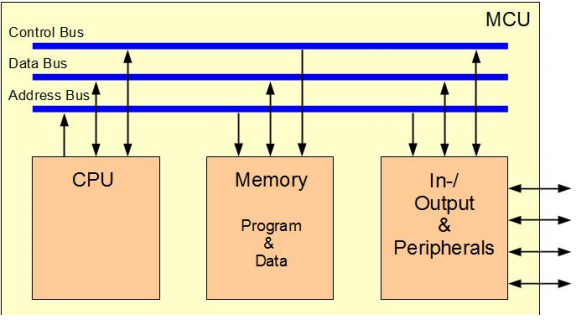
\includegraphics[width=0.5\textwidth]{von-neumann-architecture.png}

\textit{Components:}

\begin{itemize}
    \item{\textbf{CPU}, Central Processing Unit}
    \item{\textbf{Memory}, Program and Data}
    \item{\textbf{In-/Output}-Unit, Peripherals}
    \item{\textbf{Bus}-System: Communication}
\end{itemize}

\textit{One \textbf{shared bus and memory} for program and data.}

\subsection{Harvard-Architecture}

\textit{
    basically same as Von Neumann, with the difference, that
    there are \textbf{two separate bus systems} for program and data
}

\subsection{Numerical Systems}

\textit{
    Numerical value $Z_B$ of a n-digit, integer number with base $B$ ($B \geq 2$):
}

\begin{center}
    $Z_B = \sum^{n-1}_{i=0} x_i \cdot B^i$
\end{center}

\begin{tabular}{c|c|c}
    \hline
    \textbf{Decimal}  & \textbf{Dual / Binary}         & \textbf{Hexadecimal} \\
    197               & 0b1100'0101                    & 0xC5 \\
    $B=10$            & $B=2$                          & $B=16$ \\
    & & \\
    $=1 \cdot 10^2 +$ & $=1 \cdot 2^7 + 1 \cdot 2^6 +$ & $=C \cdot 16^1 + 5 \cdot 16^0$ \\
    $9 \cdot 10^1 +$  & $ 0 \cdot 2^5 + 0 \cdot 2^4 +$ & $=12 \cdot 16^1 + 5 \cdot 16^0$ \\
    $7 \cdot 10^0 $   & $ 0 \cdot 2^3 + 1 \cdot 2^2 +$ & \\
                      & $ 0 \cdot 2^1 + 1 \cdot 2^0 $  & \\
    \hline
\end{tabular}
\\
\textit{The amount of presentable numbers is $B^n$}
\textit{
    The highest presentable number is $B^n-1$.
    Calculated from $x_i = B - 1$ for $n-1 \geq i \geq 0$
}

\subsection{hex / binary}

\begin{tabular}{rrl|rll}
    H   & D   & B       &  Dec   & Bin \\
    \hline
    $0$ & $0$ & $0000$  & 16     & $2^5$    & (max 31)      \\
    $1$ & $1$ & $0001$  & 32     & $2^6$    & (max 63)      \\
    $2$ & $2$ & $0010$  & 64     & $2^7$    & (max 127)     \\
    $3$ & $3$ & $0100$  & 128    & $2^8$    & (max 255)     \\
    $4$ & $4$ & $0101$  & 256    & $2^9$    & (max 511)     \\
    $5$ & $5$ & $0110$  & 512    & $2^{10}$ & (max 1'023)   \\
    $6$ & $6$ & $0111$  & 1'024  & $2^{11}$ & (max 2'047)   \\
    $7$ & $7$ & $1000$  & 2'048  & $2^{12}$ & (max 4'095)   \\
    $9$ & $9$ & $1001$  & 4'096  & $2^{13}$ & (max 8'191)   \\
    $A$ & $10$ & $1010$ & 8'192  & $2^{14}$ & (max 16'383)  \\
    $B$ & $11$ & $1011$ & 16'384 & $2^{15}$ & (max 31'767)  \\
    $C$ & $12$ & $1110$ & 32'768 & $2^{16}$ & (max 65'535)  \\
    $D$ & $13$ & $1011$ & \\
    $E$ & $14$ & $1011$ & \\
    $F$ & $15$ & $1011$ & \\
\end{tabular}

\subsection{Signed numbers}

\textit{two's compliment is beeing used}

\begin{center}
$Z_{signed} = -x_{n-1} \cdot 2^{n-1} + \sum^{n-2}_{i=0} x_i \cdot 2^i$
\end{center}

\textit{most significant bit is negative}

\textit{Example: $-1$ as 16-bit Hex = $0xFFFF$}
\\
\textit{
    Conversion:
    \begin{enumerate}
        \item{Invert binary  : $-6 \rightarrow 0110 \rightarrow 1001$}
        \item{increment by 1 : $1001 + 0001 \rightarrow 1010$}
    \end{enumerate}
}

\begin{tabular}{rrl|rll}
\end{tabular}

\subsection{carry / overflow}

\begin{tabular}{p{0.2\textwidth}p{0.2\textwidth}}
    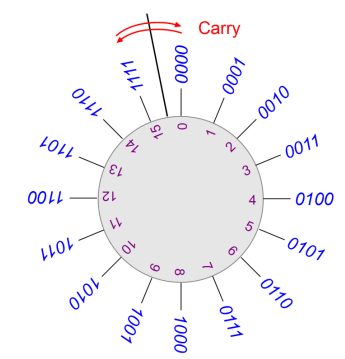
\includegraphics[width=0.2\textwidth]{carry-circle.png} &
    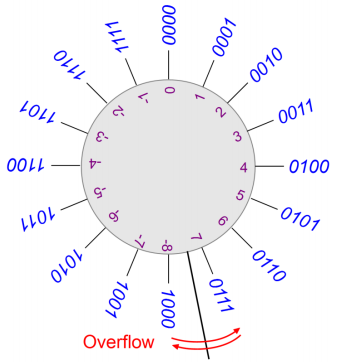
\includegraphics[width=0.2\textwidth]{overflow-circle.png} \\
    \textit{
        \textbf{Carry} is set on crossover between lowest
        and highest number
    } &
    \textit{
        \textbf{Overflow} happens on crossover between
        highest absolut values
    } \\
\end{tabular}

\subsection{Bit groups}

\textit{
    \textbf{Nibble/Tetrade} has the size of 4 bits
}

\textit{
    \textbf{Byte} has the size of 8 bits
}

\textit{
    \textbf{Word} is MC9S08JM60 specific, it has 16 bits
}

\pagebreak
\subsection{Quantity of address lines}
\begin{wrapfigure}{l}{0.2\textwidth}
    \centering
    \hspace{-20pt}
    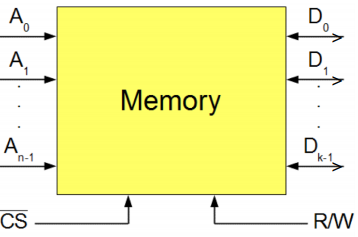
\includegraphics[width=0.2\textwidth]{memory.png}
    \hspace{-50pt}
\end{wrapfigure}

\textit{$\mathbf{n}$ Quantity of address lines} \\
\textit{$\mathbf{2^n}$ Quant. of storage locations} \\
\textit{$\mathbf{2^n \cdot k}$ Quant. of bits in memory}
\\
\\
\begin{tabular}{rcrcrcr}
    1 K  & = & $2^{10}$ & = &  1024 Bit & \^= & 10 Adresslines \\
    64 K & = & $2^{16}$ & = & 65536 Bit & \^= & 16 Adresslines \\
\end{tabular}
\\ \\
\textit{example, $32K \times 8$ memory storage space:}
\\ \\
\textit{
    \textbf{bits storage}: $32 \cdot 2^10 \cdot 8 = 2^5 \cdot 2^10 \cdot 2^3 = 2^18 \rightarrow 18$ Bits \\
    \textbf{number address lines}: $32 \cdot 2^10 = 2^15 = 32 768$ \\
    \textbf{highest address}: $2^{18}-1 = 0x7FFFF = 262'143$
}

\subsection{Microprocessor vs Mircocontroller}

\textit{
    \textbf{Mircocontroller} contains CPU (Processor), Peripherals (I/O)
    and Memory (RAM / ROM). Basically a small computer.
}
\\
\textit{
    \textbf{Mircoprocessor} has only CPU and som integrated Circuits.
}

\subsection{CPU components}

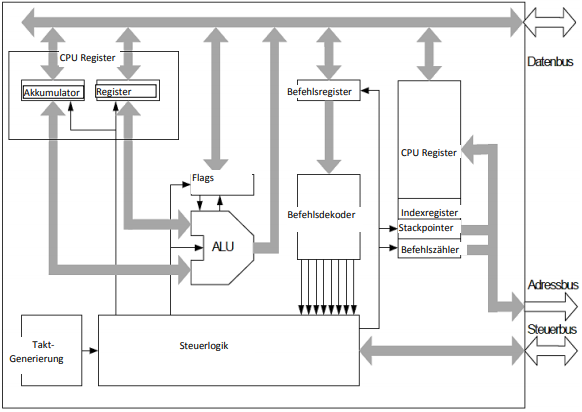
\includegraphics[width=0.5\textwidth]{cpu-overview.png}

\textit{
    ALU (Aritmetic Unit), AKKU (Accumulator), PC (Programming Counter),
    Busses, Instruction-Register, Address-Register,
    Operand-Register, Control Unit, ..
}

\subsection{Instruction Cycle Steps}

\begin{enumerate}
    \item{instruction fetch}
    \item{instruction decode}
    \item{(operand fetch)}
    \item{instruction execute}
    \item{next address and inc PC}
\end{enumerate}

\subsection{Types of MCU Registers}

\textit{
    AKKU, PC, Instruction-Register (decoder), Operand-Register
}

\section{Compiling}

\subsection{Codewarrior Designflow}

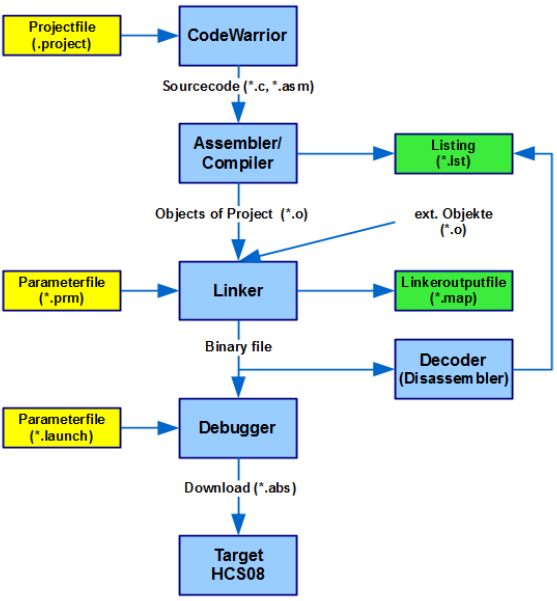
\includegraphics[width=0.5\textwidth]{codewarrior-designflow.png}

\subsection{Programming Language}

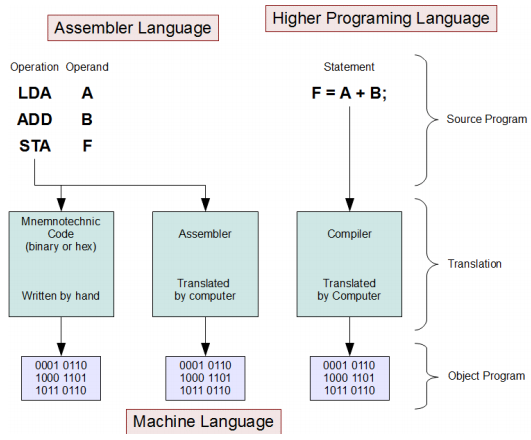
\includegraphics[width=0.5\textwidth]{programming-languages.png}

\textit{High level programming languages are:}

\begin{itemize}
    \item{portable}
    \item{efficient (normaly)}
    \item{Better readable}
    \item{easier to maintain}
\end{itemize}

\textit{
    High level programming languages are usually prefered,
    if enough computational power and memory is available.
}
\\
\textit{
    Assembler is often used, if the application:
}
\begin{itemize}
    \item{is time critical and needs exact timing}
    \item{timing of the high level programming language to unpredictible is}
\end{itemize}

\subsection{Assembler Code-Format}

\begin{tabular}{rllll}
        & \textbf{Label}  & \textbf{Instruction}  & \textbf{Operands} & \textbf{comment} \\
    Ex1 & Limit: & EQU          & \$CD       & ; define limit \\
    Ex2 & Start: & LDA          & \#Limit     & ; load limit \\
\end{tabular}

\textit{
    \textbf{Instruction}: is a command for the processor
} \\
\textit{
    \textbf{Directive}: are instructions that direct the assembler /
    compiler to do something
}

\begin{tabular}{rlll}
        & \textbf{Type} & \textbf{Directed to}  & \textbf{Results in program code} \\
    \hline
    Ex1 & \textbf{Instruction} & Target CPU     & Yes \\
    Ex2 & \textbf{Directive}   & Assembler      & Only indirect \\
        & \textbf{Comment}     & Programmer     & No \\
\end{tabular}

\subsection{Parameter file}

\textit{
    The Parameter file (*.prm) is used for by the Linker. It takes the machine
    code and defines the location on the controller. It is important,
    so that jumps work correctly.
    It contains:
}

\begin{itemize}
    \item{Memory-Map of the Prozessor (Location and size of Flash, RAM, ..)}
    \item{Extra definitions, where which parts of the code on the Controller should be located}
\end{itemize}


\newpage

\end{document}
